\chapter{RESULTADOS E DISCUSSÃO}\label{CAP4}

\section{RESULTADOS EXPERIMENTAIS}
Os resultados experimentais obtidos para o ensaio de Mancha de Areia estão contidos na Tabela \ref{tab:manchadeareia_resultados}, a seguir. Os valores médios de MDT encontrados foram 1,000 e 1,035 para concreto e asfalto, respectivamente. 

\begin{table}[htb!]
\centering
\caption{Resultado dos ensaios experimentais de Mancha de Areia.}
\label{tab:manchadeareia_resultados}
\begin{tabular}{cc}
\hline
Corpo de Prova & \multicolumn{1}{c}{MDT} \\ \hline
1              & 0.998                            \\
2              & 1.002                            \\
3              & 0.770                            \\
4              & 1.300                            \\ \hline
\end{tabular}
\end{table}

Foi realizada a classificação da macrotextura de acordo com a Tabela \ref{tab:alturadeareia} extraída do \citeonline{dnit031}, concluindo-se que ambos os pavimentos apresentam textura grosseira ou aberta. Observou-se também que os valores de MDT encontram-se dentro dos limites sugeridos pelo DNIT (1,20mm $\geq$ HS $\geq$ 0,60mm), atendendo aos requisitos de segurança. Quanto a resistência à derrapagem, os pavimentos apresentam classificação rugosa (Tabela \ref{tab:resistencia}).

\section{RESULTADOS COMPUTACIONAIS}
O scanner conseguiu representar de forma satisfatória as superfícies dos pavimentos, como pode ser observado nas Figuras \ref{Fig:6leituras} e \ref{Fig:3leituras}. Os dados retornados pelo escaneamento apresentam detalhes visualmente precisos em relação textura os corpos de prova, de forma que o algoritmo possa ajustar as profundidades próximas das experimentais.

\begin{figure}[!ht]
\centering
{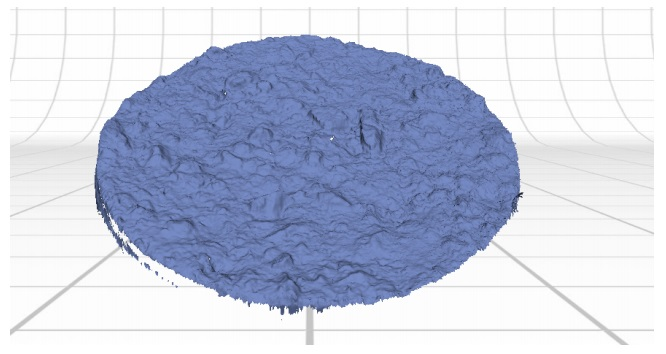
\includegraphics[scale=0.83]{figures/6leituras.jpg}}\\
\caption{Perfilamento tridimensional com 6 leituras do pavimento asfáltico.}
\makebox[\width]{Representação da nuvem de pontos retornada pelo scanner.} 
\label{Fig:6leituras}
\end{figure}

\begin{figure}[!ht]
\centering
{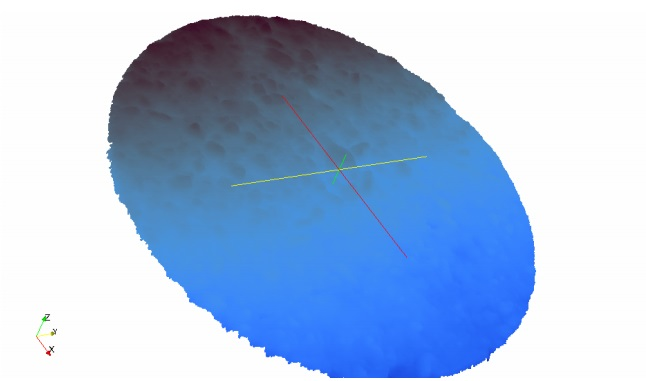
\includegraphics[scale=0.83]{figures/3leituras.jpg}}\\
\caption{Perfilamento tridimensional com 3 leituras do pavimento asfáltico.}
\makebox[\width]{Representação após o tratamento para retirada de pontos atípicos.}
\label{Fig:3leituras}
\end{figure}

As representações das superfícies dos quatro pavimentos obtidas a partir do escaneamento tridimensional estão representadas na Figura \ref{Fig:cps}. Por meio de uma avaliação visual das representações das superfícies obtidas, nota-se que o pavimento asfáltico é significativamente mais rugoso do que pavimento rígido de concreto.

\begin{figure}[!ht]
\centering
\subfigure[ref1][CP1]
{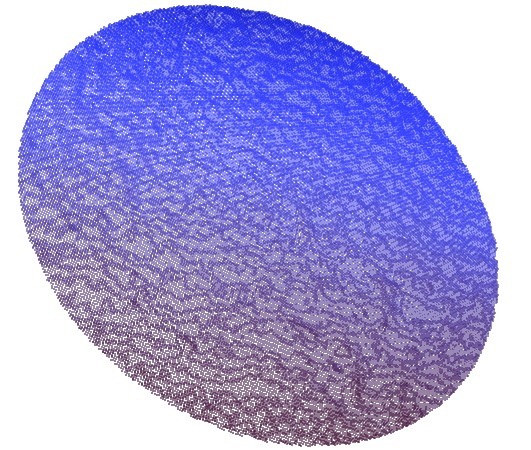
\includegraphics[scale=0.5]{figures/cp1.jpg}}
\qquad
\subfigure[ref2][CP2]{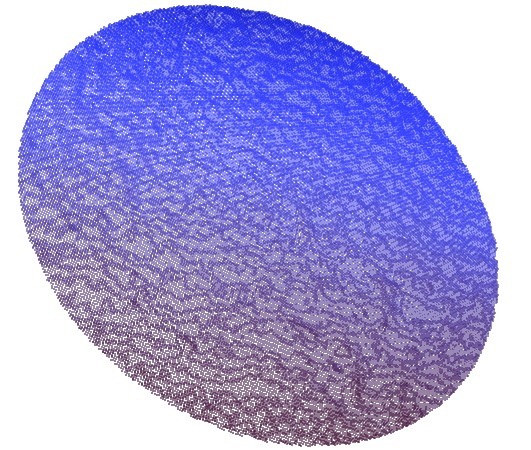
\includegraphics[scale=0.5]{figures/cp2.jpg}}\\
\subfigure[ref2][CP3]
{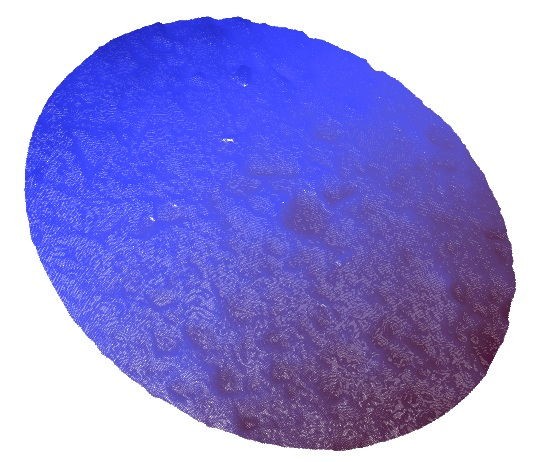
\includegraphics[scale=0.50]{figures/cp3.jpg}}
\subfigure[ref2][CP4]
{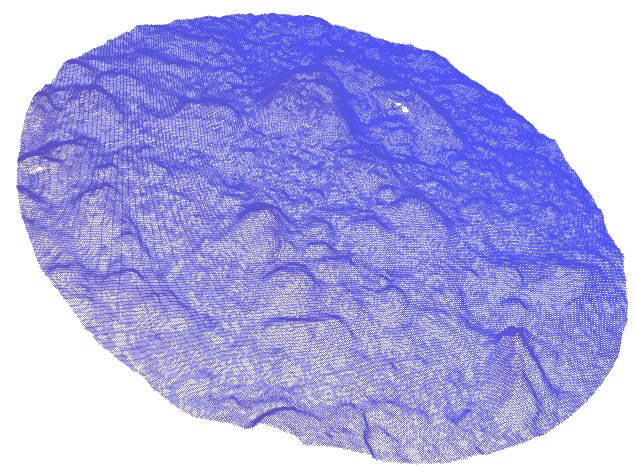
\includegraphics[scale=0.44]{figures/cp4.jpg}}
\caption{Representação das superfícies escaneadas.}\makebox[\width]{(a) e (b) referem-se às amostras de concreto; (c) e (d) às amostras de asfalto.} 
\label{Fig:cps}
\end{figure}

O algoritmo realizou as aproximações das Profundidades Médias do Perfil (MPD) cujos resultados constam na Tabela \ref{tab:resultadoscomputacionais}, assim como os erros em relação aos resultados experimentais. 

\begin{table}[htb!]
\centering
\caption{Resultados estimados de MTD e erros em relação aos valores experimentais}
\label{tab:resultadoscomputacionais}
\begin{tabular}{ccccc}
\hline
\multirow{2}{*}{Rótulo} & \multicolumn{2}{c}{3 leituras}                                        & \multicolumn{2}{c}{6 leituras}                                        \\ \cline{2-5} 
                        & \multicolumn{1}{c}{Estimado} & \multicolumn{1}{c}{Erro Relativo (\%)} & \multicolumn{1}{c}{Estimado} & \multicolumn{1}{c}{Erro Relativo (\%)} \\ \hline
1                       & 1.012                        & 1.40                                   & 1.052                        & 5.41                                   \\
2                       & 1.001                        & 0.10                                   & 1.022                        & 1.99                                   \\
3                       & 0.792                        & 2.83                                   & 0.783                        & 1.70                                   \\
4                       & 1.285                        & 1.12                                   & 1.308                        & 0.61                                   \\ \hline
\end{tabular}
\end{table}

\section{ANÁLISE DOS RESULTADOS}

As respostas do algoritmo foram bastante próximas dos valores experimentais. Embora tenha-se observado uma grande variação nos erros relativos, estes apresentaram valores aceitáveis, sendo o máximo erro 2,83\% para 3 leituras e 5,41\% para 6 leituras. 

Observou-se também que os resultados foram condizentes entre si. Contudo, nos ensaios experimentais foi encontrada uma grande variação entre valores de MTD para os corpos de prova de asfalto (aproximadamente 70\%), indicando que este resultado médio não é muito apurado. Também cabe ressaltar que apesar da análise visual indicar que o pavimento asfáltico é bem menos rugoso que o pavimento de concreto, a diferença númerica entre os valores de MTD não foi tão significativa. Assim, presume-se que caso mais medidas fossem realizadas o valor de MTD para os pavimentos asfálticos seria reduzido.  

O desvio padrão ficou em torno de 0.25, de forma que os ajustes das profundidades realizados nos planos transversais se distanciam pouco da média. A mediana se aproximou da média estimada pelo algoritmo mostrando que as distribuições das profundidades foram aproximadamente simétricas. A curtose com valores maiores que zero indica uma distribuição mais alta e concentrada do que a curva normal, se tratando de uma função leptocúrtica, enquanto os resultados menores que zero se referem a uma fução mais achatada, chamada platicúrtica \cite{magalhaes}.

\begin{table}[htb!]
\centering
\caption{Valores estimados para os parâmetros descritivos desvio padrão, mediana e curtose.}
\label{tab:parametrosDescritivos}
\begin{tabular}{crrrrrr}
\hline
\multirow{2}{*}{Corpo de Prova} & \multicolumn{2}{c}{Desvio Padrão}                               & \multicolumn{2}{c}{Mediana}                                     & \multicolumn{2}{c}{Curtose}                                     \\ \cline{2-7} 
                                & \multicolumn{1}{c}{3 leituras} & \multicolumn{1}{c}{6 leituras} & \multicolumn{1}{c}{3 leituras} & \multicolumn{1}{c}{6 leituras} & \multicolumn{1}{c}{3 leituras} & \multicolumn{1}{c}{6 leituras} \\ \hline
1                               & 0.250                          & 0.323                          & 1.021                          & 0.993                          & 1.051                          & 3.911                          \\
2                               & 0.179                          & 0.205                          & 1.010                           & 0.950                          & -0.204                         & 0.306                          \\
3                               & 0.188                          & 0.144                          & 0.782                          & 0.760                          & -0.253                         & 5.199                          \\
4                               & 0.334                          & 0.319                          & 1.239                          & 1.375                          & -0.948                         & -0.618                         \\ \hline
\end{tabular}
\end{table}

Para melhor visualização dos resultados, foi traçado o gráfico da Profundidade Média do Perfil (MPD), parâmetro obtido computacionalmente \emph{versus} Textura Média do Pavimento (MDT), obtida experimentalmente (Figura \ref{Fig:grafico}). Os dados contidos no gráfico referem-se a cada um dos oito ensaios realizados. 

\begin{figure}[!ht]
\centering
{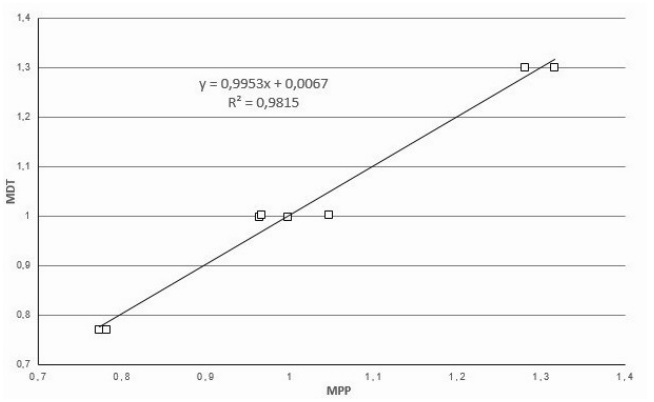
\includegraphics[scale=0.83]{figures/grafico.jpg}}\\
\caption{Relação Profundidade Média do Perfil (MPD) e Textura Média do Pavimento (MDT).} 
\label{Fig:grafico}
\end{figure}

A equação representativa dos resultados encontra-se representada e o coeficiente de correlação encontrado foi (R$^2=0,9815$), o que indica uma forte correlação entre MPD e MDT. 


